\documentclass{beamer}
\usepackage{lmodern}
\usepackage{HECbeamer} 
% \usepackage{pgfpages}
% \pgfpagesuselayout{4 on 1}[letterpaper, landscape, border shrink=5mm]
\title[\color{white}{MATH60604A Predictions}]{\texorpdfstring{MATH60604A \\Statistical modelling \\ \S 2f - Predictions}{MATH60604A \\Statistical modelling \\ \S~2f - Predictions}}
\author{Léo Belzile}
\institute{HEC Montréal\\
Department of Decision Sciences}
\date{} 
% \newcommand{\AIC}{\ensuremath{\mathsf{AIC}}}
% \newcommand{\BIC}{\ensuremath{\mathsf{BIC}}}
\begin{document}
\frame{\titlepage}

\begin{frame}
\frametitle{Predicted and fitted values}
\bi
\item In many applications, particularly in database marketing, the primary goal is to develop a model to get predictions of the dependent variable and use them to make business decisions.
\item For example, we might want to predict the amount of money spent if we were to send an offer to a client. 
\item The usual way of proceeding would be to send offers to a sample of clients, build a model with the data, then apply the model (i.e., obtain predictions) for the other clients in the dataset. 
\ei
\end{frame}



\begin{frame}
\frametitle{Prediction}
\bi
\item We may want to estimate the \alert{mean value of $Y$} when $\mathbf{X}=\bs{x}$,
\begin{align*}
\E{Y\mid \mathbf{X}=\bs{x}}=\beta_0+\beta_1x_1 + \cdots + \beta_px_p.\end{align*}
\item We also might want to \alert{predict the value} of a new random variable $Y_i$ when $\mathbf{X}_i=\bs{x}$; recall that 
\begin{align*}
Y_i=\beta_0+\beta_1x_1 + \cdots + \beta_px_p +\varepsilon_i.
\end{align*}
\item Whether we want to predict the \alert{mean} or the \alert{value} of $Y$ when $\mathbf{X}=\bs{x}$, the predicted values will be the point on the ``line'' corresponding to $\mathbf{X}=\bs{x}$,
\begin{align*}
\hat{\beta}_0+\hat{\beta}_1x_{1} + \cdots + \hat{\beta}_px_{p}.
\end{align*}

\ei

\end{frame}
\begin{frame}
\frametitle{Individual predictions are more uncertain}
\bi 
\item The mean prediction and the prediction for an individual value are the \textbf{same} for the linear regression.
\bi \item we will see later that this is not the case for mixed models, in which there are random effects for individuals or groups
\ei
\item While the estimator of the mean of $Y$, $\E{Y \mid \mathbf{X}}$ will be the same, it will be \alert{\textbf{more precise}} than the prediction of an individual value $Y_i$.
\item The \textbf{confidence interval} (for the mean) would be smaller than the \textbf{prediction interval}.
\bi \item \textbf{rationale}: additional uncertainty due to $\eps$ for the new observation.
\ei
\item Once the parameters have been estimated, we can get predicted/fitted values for
$Y$ for a given set of predictors $\mathrm{X}_1=x_1, \ldots,\mathrm{X}_p=x_p$
\begin{align*}
\hat{Y}=\hat{\beta}_0 +\hat{\beta}_1 x_1+\ldots+\hat{\beta}_px_p.
\end{align*}
\ei
\end{frame}

\begin{frame}[fragile]
\frametitle{Predicted values and prediction intervals in \SASlang}
\bi
\item We will start by creating a new dataset \code{newdata} containing the values of the explanatory variables we want to make predictions for. 
\item We use the first observation and copy all of the explanatories from that individual, but change fixation so that it varies from $0$ to $6$ seconds.
\ei
\begin{tcolorbox}[colback=white, colframe=hecblue, title=\SASlang code to create a new dataset \code{newdata} ]
\begin{verbatim}
data newdata;
   set statmod.intention(obs=1);
   do fixation=0 to 6;
      output;
   end;
run;
\end{verbatim}
\end{tcolorbox}
\end{frame}

\begin{frame}[fragile]
\frametitle{Saving the output of the linear model for prediction}
\bi
\item Next, we fit the linear model and save the information needed in order to make predictions in an object, say \code{modelinfo}.
\item Next, we use the procedure \code{plm} to get predictions from the object \code{modelinfo}. These predictions will be saved in the temporary file \code{prediction}.
\item We also ask for confidence intervals for both the mean (\code{lclm} and \code{uclm}) and individual predictions (\code{lcl} and \code{ucl}).
\ei
\begin{tcolorbox}[colback=white, colframe=hecblue, title=\SASlang code to save fit of linear models]
{\small
\begin{verbatim}
proc glm data=statmod.intention noprint;
class sex educ revenue;
model intention= fixation emotion 
    sex age revenue educ / ss3 solution;
store modelinfo; 
run;
\end{verbatim}
}
\end{tcolorbox}
\end{frame}

\begin{frame}[fragile]

\begin{tcolorbox}[colback=white, colframe=hecblue, title=\SASlang code to get predictions using \code{plm} ]
\begin{verbatim}
proc plm restore=modelinfo; 
score data=newdata out=prediction predicted 
    lclm uclm lcl ucl; 
run;

proc sgplot data=prediction;
band x=fixation upper=ucl lower=lcl / 
        fill transparency=.5 
        legendlabel="individual";
band x=fixation upper=uclm lower=lclm / 
        fill transparency=.1 legendlabel="mean";
series x=fixation y=predicted;
yaxis label="intention score";
xaxis label="fixation time (in seconds)";
run;
\end{verbatim}
\end{tcolorbox}
\end{frame}


\begin{frame}[fragile]
\frametitle{Confidence bands for the mean and prediction bands}
\begin{center}
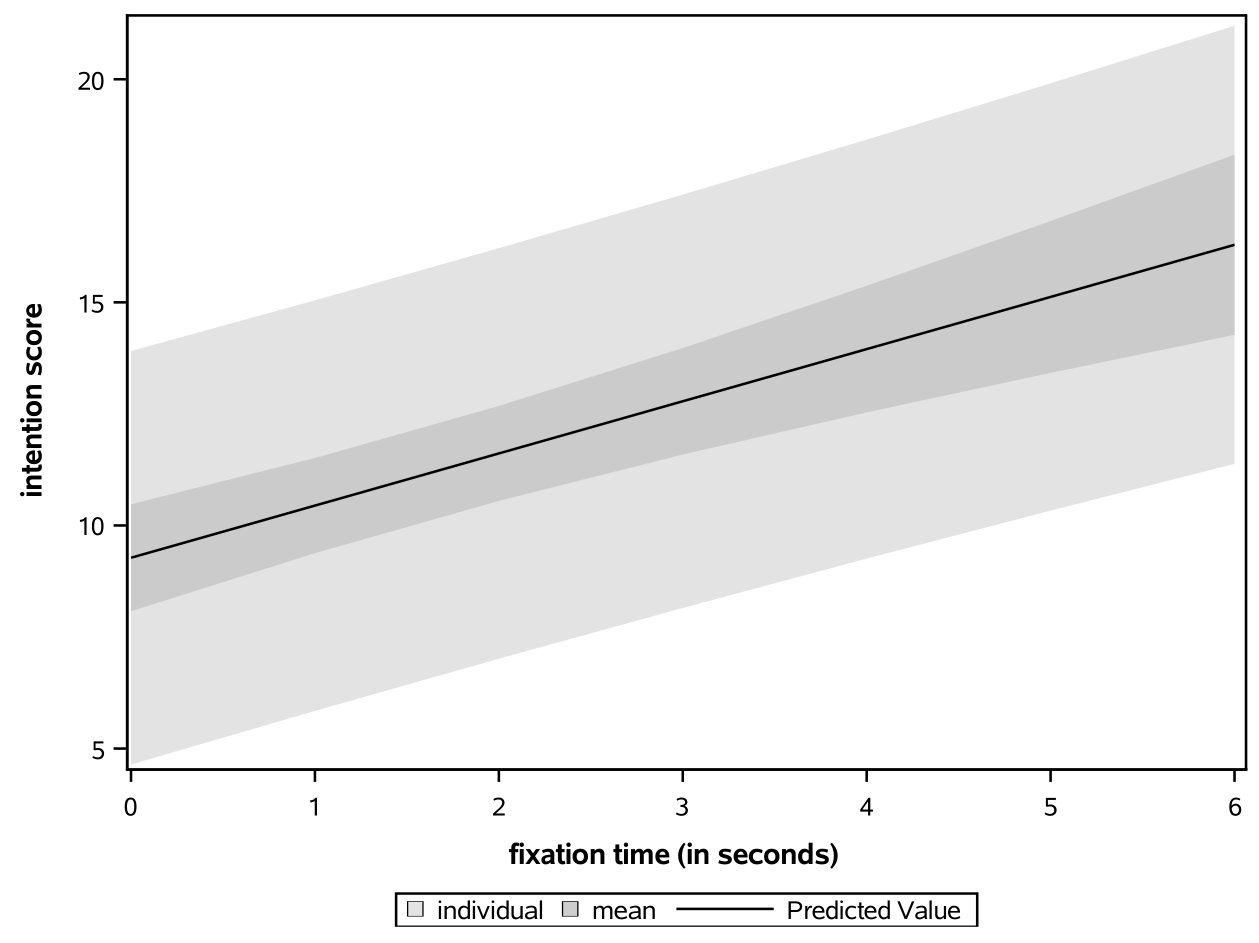
\includegraphics[width = 0.75\linewidth]{img/c2/slides3-e17}
\end{center}
{\footnotesize The prediction bands (light gray) are wider than the confidence bands for the mean (dark gray). The prediction and confidence intervals get wider when we move away from the mean value of \code{fixation}

}
\end{frame}
  \end{document}
